%% selection_pressure.tex
%% Author: Leighton Pritchard
%% Copyright: James Hutton Institute
%% A brief introduction to orthologues, and their prediction

%
\begin{frame}
  \frametitle{Selection Pressure
  }
  \Large{
    \textcolor{olive}{
      \textbf{
      Comparative genomics helps identify selection pressures at a structural and sequence level
      }
    }
  }
\end{frame}

%
\begin{frame}
  \frametitle{How orthologues help}
  \textcolor{hutton_green}{Defining core groups of genes as ``orthologue`'' allows analysis of groups of genes together by:}
  \begin{itemize}
    \item \textcolor{hutton_purple}{synteny/collocation}
    \item gene neighbourhood changes (e.g. \textcolor{hutton_purple}{\textit{genome expansion}})
    \item \textcolor{hutton_purple}{pan genome (core/accessory genomes)}
  \end{itemize}
  \textcolor{hutton_blue}{and of individual genes within those groups, by:}
  \begin{itemize}
    \item multiple alignment
    \item domain detection
    \item identification of functional sites
    \item \textcolor{hutton_purple}{inference of evolutionary pressure}
  \end{itemize}  
\end{frame}

%
\begin{frame}
  \frametitle{Synteny
    \footnote{\tiny{Alvarez-Ponce \textit{et al}. (2011) \textit{Genome Biol. Evol.} \href{http://dx.doi.org/10.1093/gbe/evq084}{doi:10.1093/gbe/evq084
  }}}
}
  Selection pressures depend on gene (product) function
  \begin{itemize}
    \item \textcolor{hutton_green}{Genes involving physically or functionally-interacting proteins tend to involve under selective constraints} \\
    In bacteria, this leads to coexpression in \textit{regions} and collocation in \textit{operons}
    \item \textcolor{hutton_blue}{Collocation (and correlation) may be identified by genome comparisons}
    \item \textcolor{RawSienna}{Also true for regulatory and metabolic networks}
  \end{itemize}  
\end{frame}

%
\begin{frame}
  \frametitle{Synteny
    \footnote{\tiny{Soderlund \textit{et al}. (2011) \textit{Nucl. Acids Res.} \href{http://dx.doi.org/10.1093/nar/gkr123}{doi:10.1093/nar/gkr123
  }}}
    \footnote{\tiny{Proost \textit{et al}. (2011) \textit{Nucl. Acids Res.} \href{http://dx.doi.org/10..1093/nar/gkr955}{doi:1093/nar/gkr955
  }}}
}
  Several tools for synteny detection, e.g.
  \begin{columns}[T] 
    \column{.6\textwidth}   
      \begin{itemize}
        \item \textcolor{hutton_green}{SyMAP {\tiny\href{http://www.agcol.arizona.edu/software/symap/}{http://www.agcol.arizona.edu/software/symap/}}}
        \item \textcolor{hutton_blue}{i-ADHoRe {\tiny\href{http://bioinformatics.psb.ugent.be/software/details/i-ADHoRe}{http://bioinformatics.psb.ugent.be/software/details/i-ADHoRe}}}
        \item MCScan, Cyntenator, etc.  
      \end{itemize}  
      \column{.4\textwidth}
        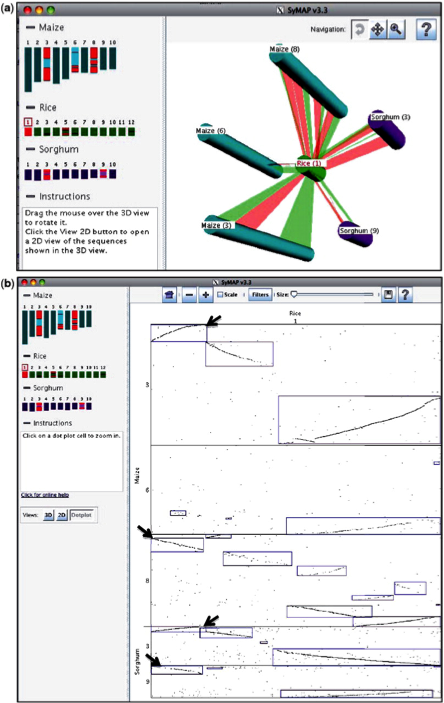
\includegraphics[height=0.6\textheight]{images/symap}
    \end{columns}
\end{frame}

%
\begin{frame}
  \frametitle{i-ADHoRe
    \footnote{\tiny{Proost \textit{et al}. (2011) \textit{Nucl. Acids Res.} \href{http://dx.doi.org/10..1093/nar/gkr955}{doi:1093/nar/gkr955
  }}}
}
  Algorithm: starts from defined equivalent genes to produce genome-scale multiple alignments of blocks of genes
  {\small
  \begin{columns}[T] 
    \column{.4\textwidth}   
      \begin{enumerate}
        \item Combine tandem repeats of gene sets
        \item Make \textcolor{hutton_green}{\textit{gene homology matrix} (GHM)}
        \item Convert collinear GHMs to \textcolor{hutton_blue}{\textit{profiles}}
        \item Align \textit{profiles} (GG2 algorithm)
        \item Search next genome with profiles, and \textcolor{hutton_purple}{iterate until complete}
      \end{enumerate}  
      \column{.6\textwidth}
        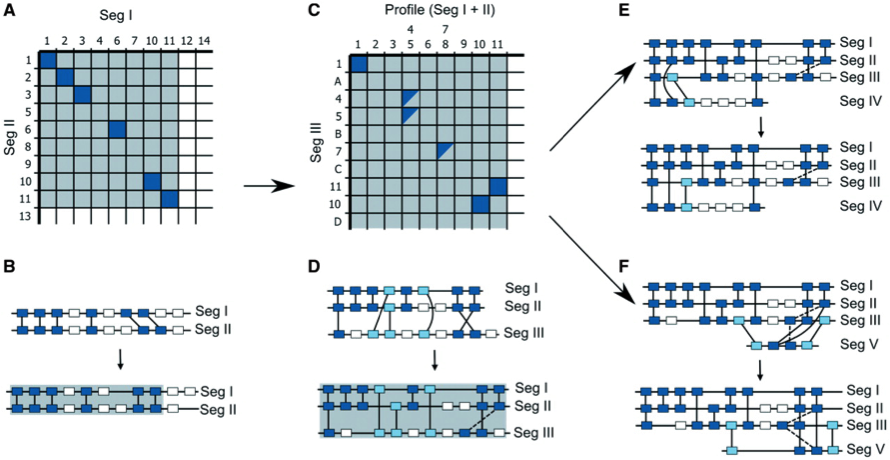
\includegraphics[width=\textwidth]{images/i-adhore_algorithm}
    \end{columns}
    }    
\end{frame}

%
\begin{frame}
  \frametitle{Finding ``Orthologues'': RBBH}
  \Large{
    \textcolor{hutton_blue}{
      \textbf{
      EXERCISE 10: \\
      \texttt{i-ADHoRe/ex10a\_i-ADHoRe.md}      
      \texttt{i-ADHoRe/ex10b\_i-ADHoRe.ipynb}
      }
    }
  }
\end{frame}